\section{Q4}
\label{part4}
\begin{enumerate}

\item 3.1 Choose a news-related event

\item 3.2 Use twarc.py to collect 1000 tweets, every day for 5 different days
\subitem - See: \url{https://github.com/edsu/twarc}

\item 3.3 For each day:
\subitem - Create a wall
\subitem - Build a tag/word cloud for each day
\subitem - Create a map using GeoJSON and Github
\subsubitem - See: \url{https://help.github.com/articles/mapping-geojson-files-on-github/}

\item 3.4 Discuss in detail lessons learned, experiences, etc.

\end{enumerate}



\subsection{Solution}
\begin{enumerate}

\item I wrote a python program using `Twarc' library to collect daily 1000 tweets.
\item The news-related event that I chose was ``Nepal Earthquake".
\item Once I was done collecting the tweets, I used different tools in the Twarc package to get the wall, word cloud and geojson from these saved tweets.
\item Wall is a HTML document displaying the tweets with user handle, Tweet text, displays URLs if any, date time of the Tweet and displays the number of retweets.
\item Word Cloud is a HTML document which displays the cloud of most frequently used words in the list of tweets and displays these words as an image beautifully.
\item GeoJSON tool gives the locations from where the Tweet originated. It can give the location only if the Tweet has location information. Using this location information, github.com plots these on map.
\item Following are the screenshots of walls, word clouds and geojsons for 5 different days.

\newpage
\subsubsection{Walls}
\begin{figure}[ht]    
    \begin{center}
        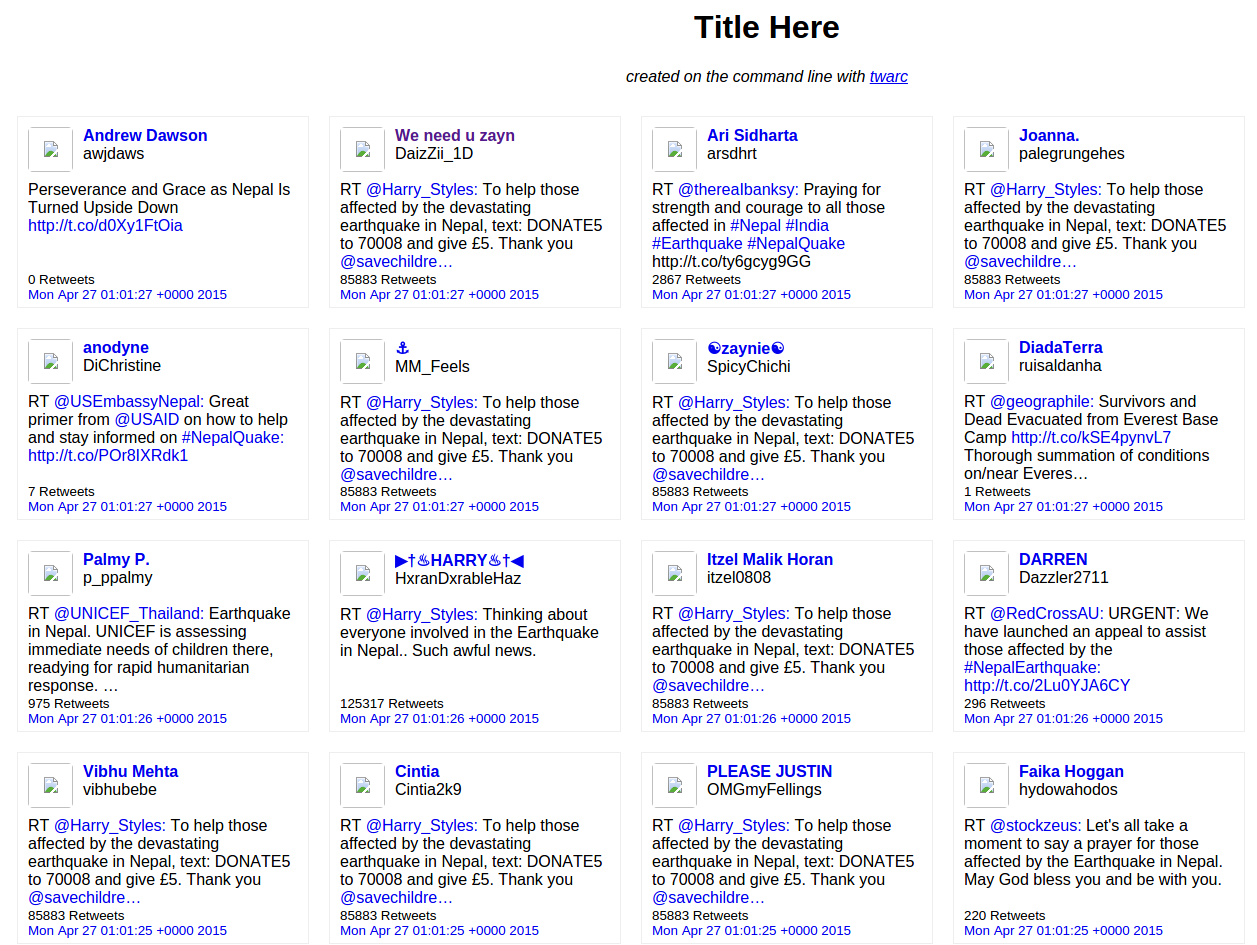
\includegraphics[scale=0.40]{graphs/wall1.png}
        \caption{Wall 1}
    \end{center}
\end{figure}

\newpage
\begin{figure}[ht]    
    \begin{center}
        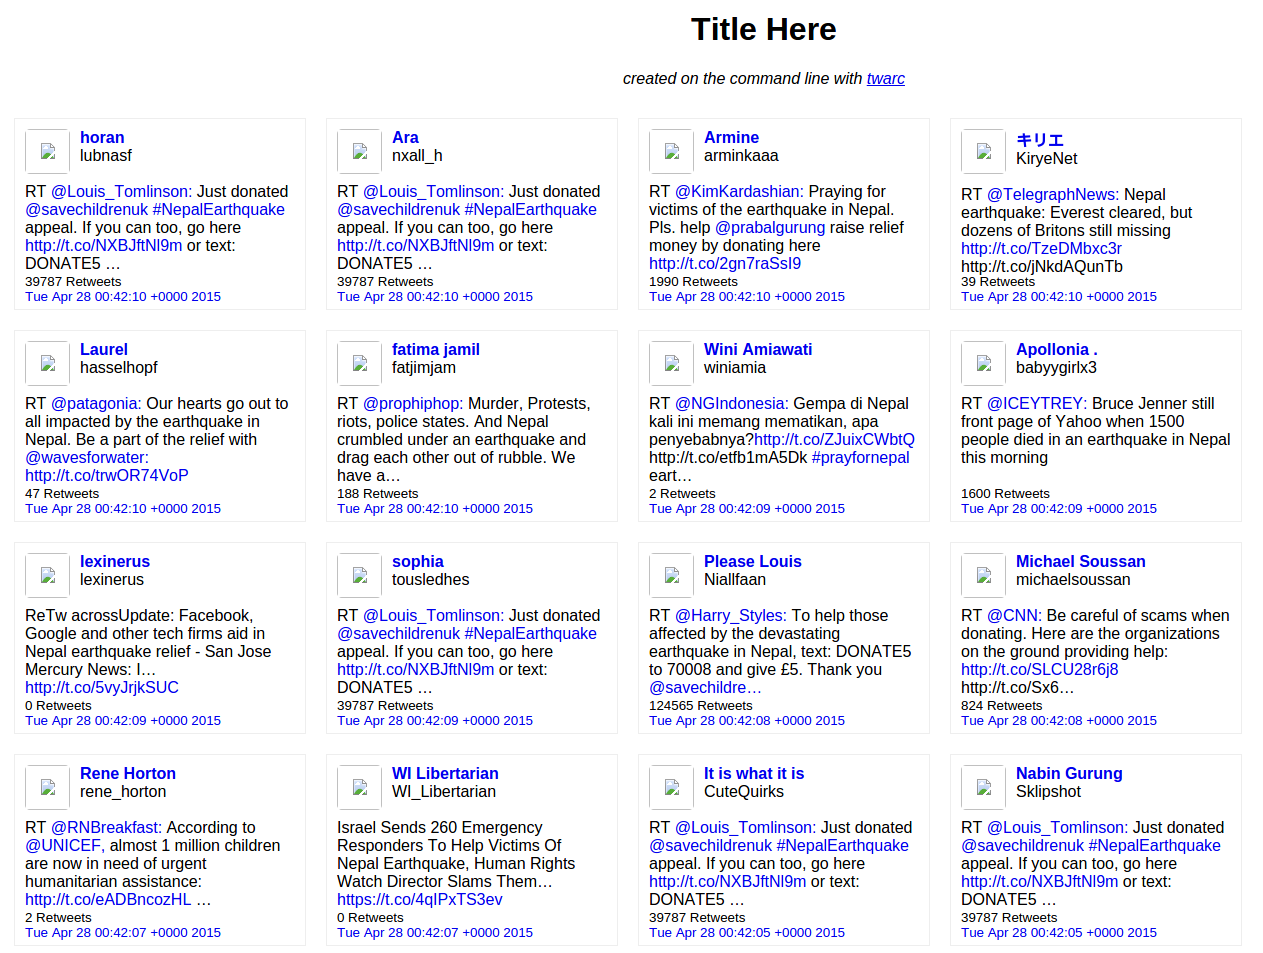
\includegraphics[scale=0.40]{graphs/wall2.png}
        \caption{Wall 2}
    \end{center}
\end{figure}

\newpage
\begin{figure}[ht]    
    \begin{center}
        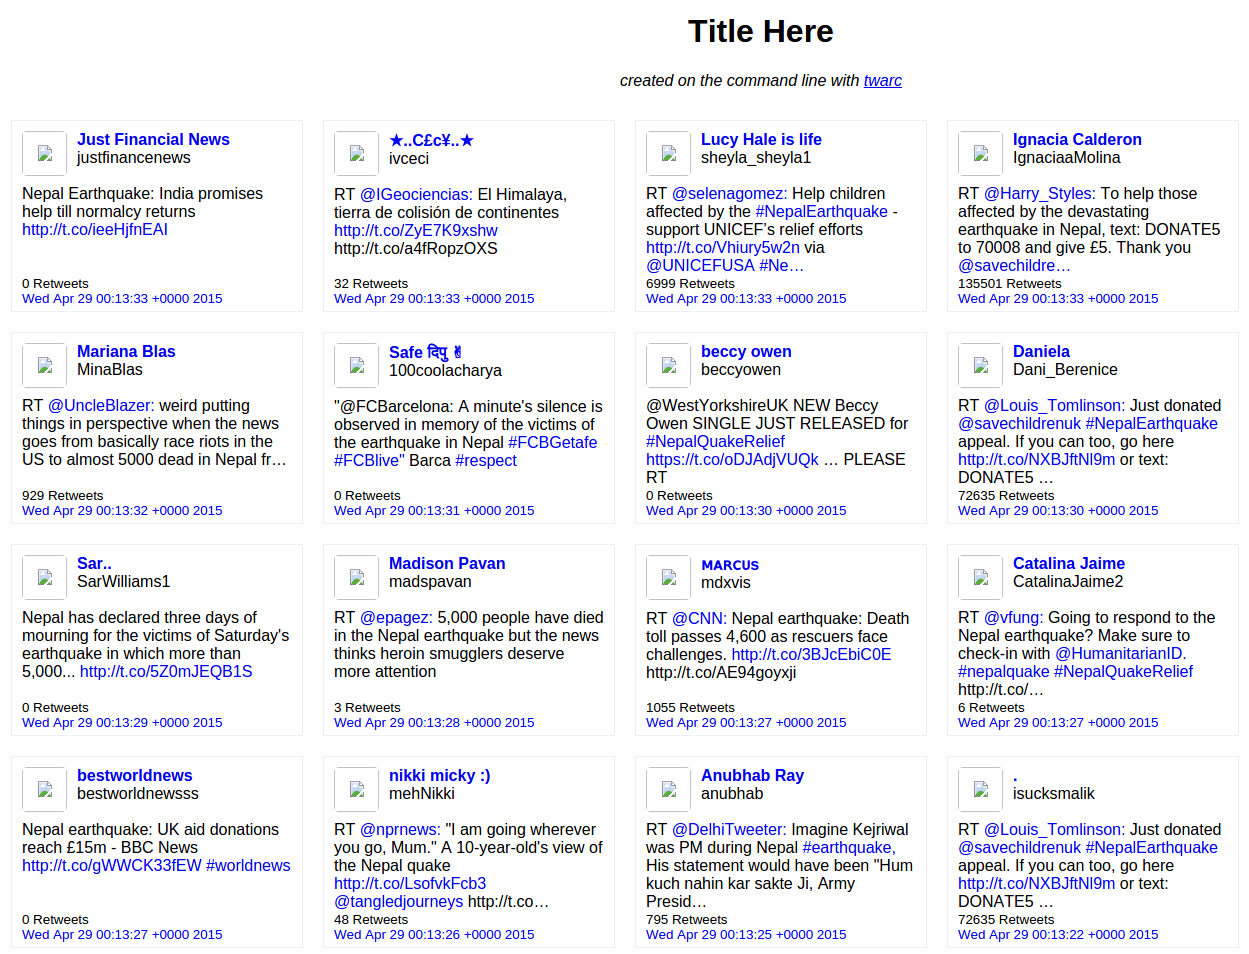
\includegraphics[scale=0.40]{graphs/wall3.png}
        \caption{Wall 3}
    \end{center}
\end{figure}

\newpage
\begin{figure}[ht]    
    \begin{center}
        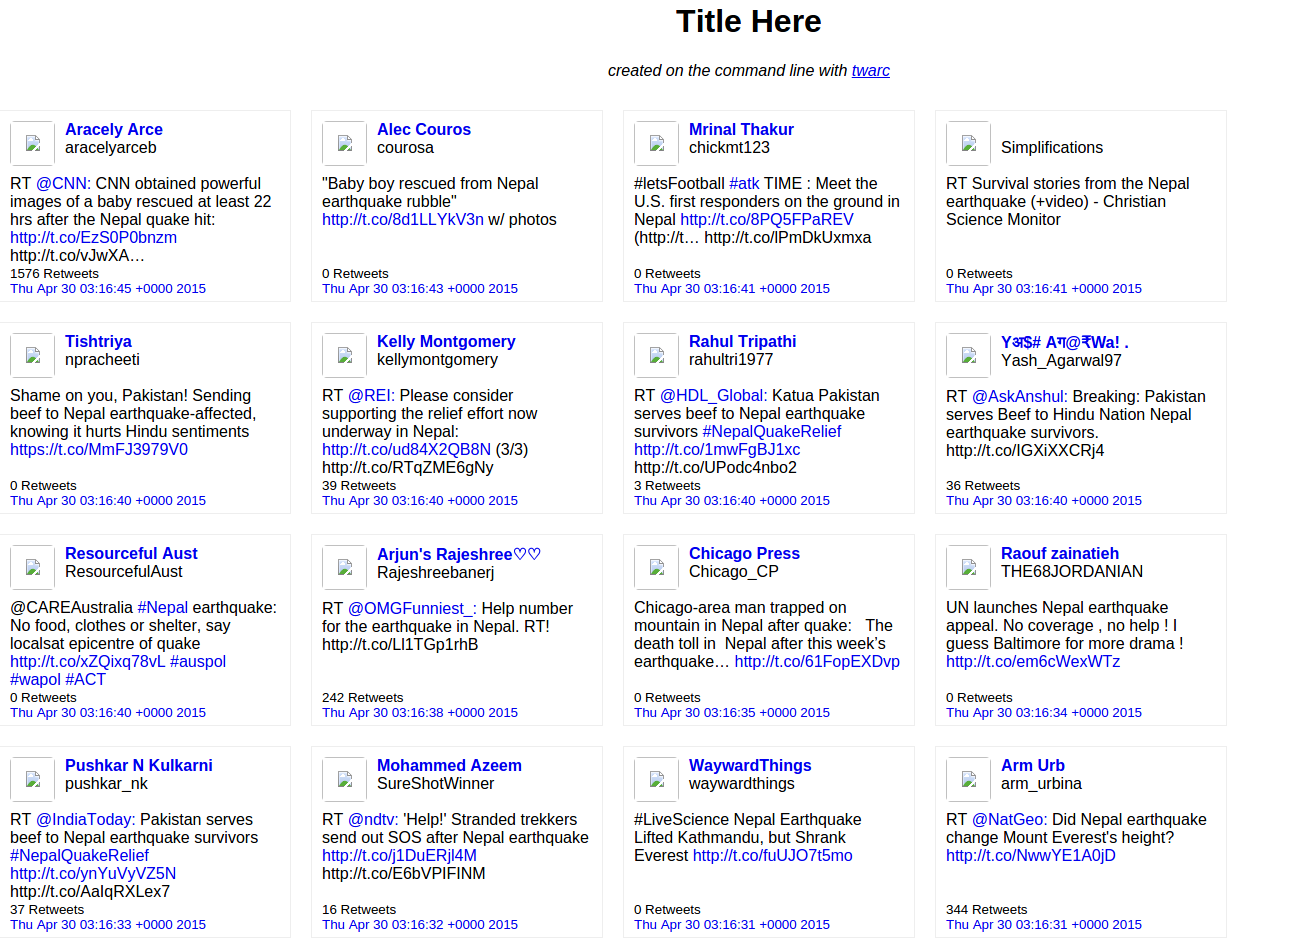
\includegraphics[scale=0.40]{graphs/wall4.png}
        \caption{Wall 4}
    \end{center}
\end{figure}

\newpage
\begin{figure}[ht]    
    \begin{center}
        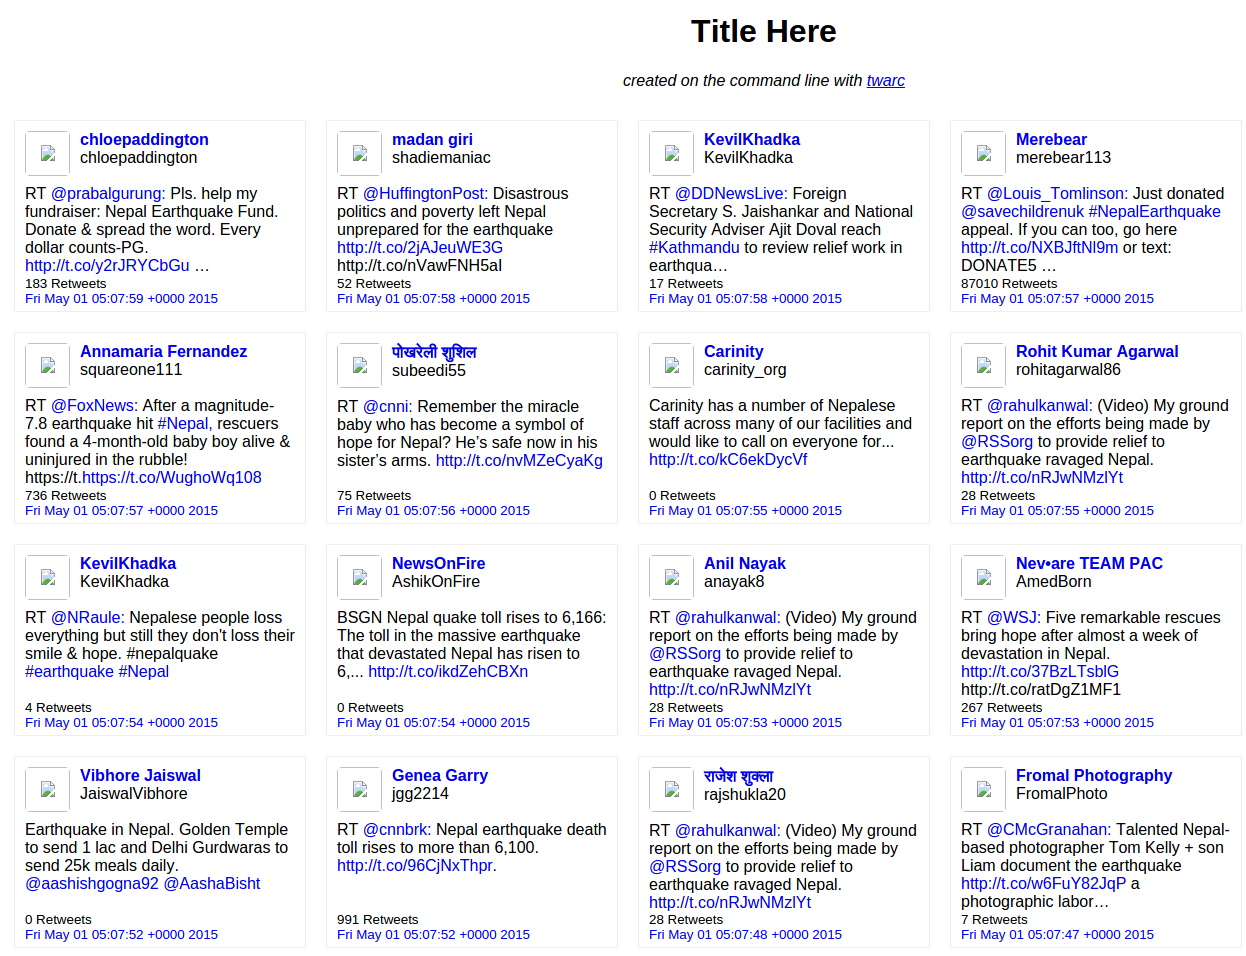
\includegraphics[scale=0.40]{graphs/wall5.png}
        \caption{Wall 5}
    \end{center}
\end{figure}

\newpage
\subsubsection{Word Clouds}
\begin{figure}[ht]    
    \begin{center}
        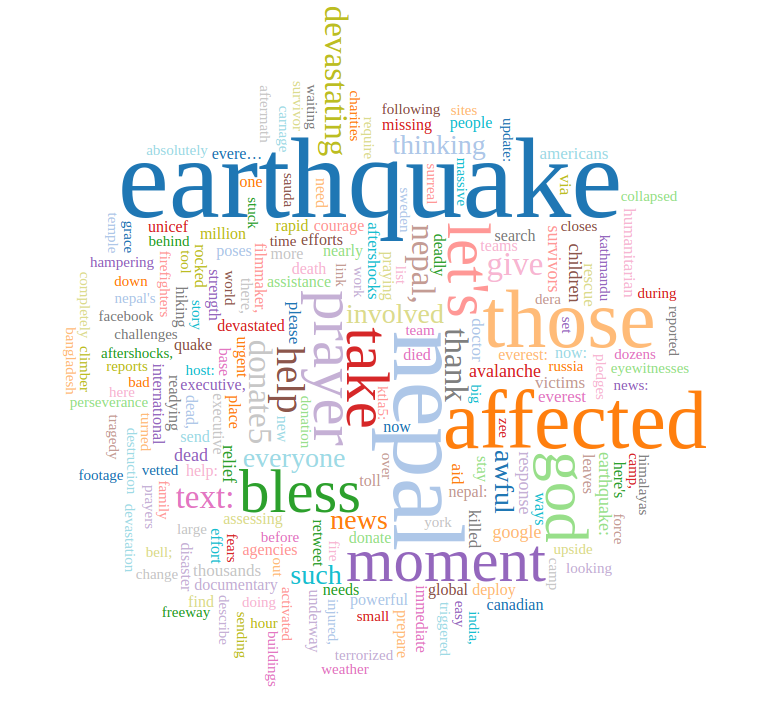
\includegraphics[scale=0.40]{graphs/wc1.png}
        \caption{Word Cloud 1}
    \end{center}
\end{figure}

\newpage
\begin{figure}[ht]    
    \begin{center}
        
\includegraphics[scale=0.40]{graphs/wc2.png}
        \caption{Word Cloud 2}
    \end{center}
\end{figure}

\newpage
\begin{figure}[ht]    
    \begin{center}
        
\includegraphics[scale=0.40]{graphs/wc3.png}
        \caption{Word Cloud 3}
    \end{center}
\end{figure}

\newpage
\begin{figure}[ht]    
    \begin{center}
        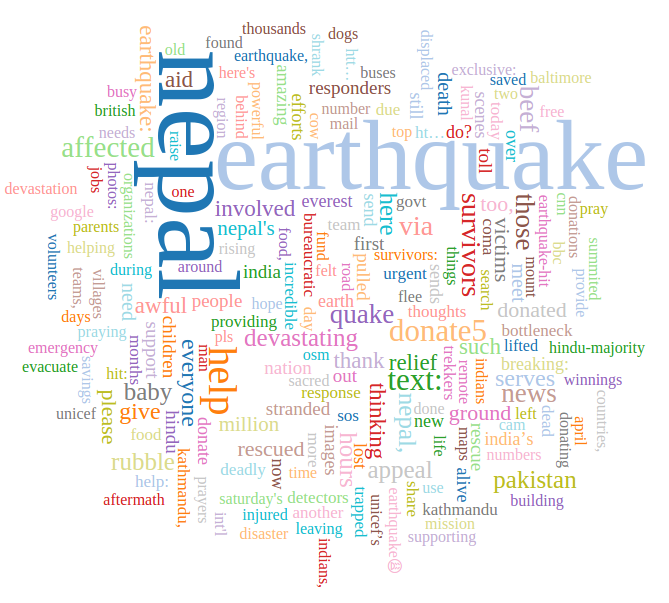
\includegraphics[scale=0.40]{graphs/wc4.png}
        \caption{Word Cloud 4}
    \end{center}
\end{figure}

\newpage
\begin{figure}[ht]    
    \begin{center}
        
\includegraphics[scale=0.40]{graphs/wc5.png}
        \caption{Word Cloud 5}
    \end{center}
\end{figure}

\newpage
\newpage
\newpage
\subsubsection{GeoJSONs}
\begin{figure}[ht]    
    \begin{center}
        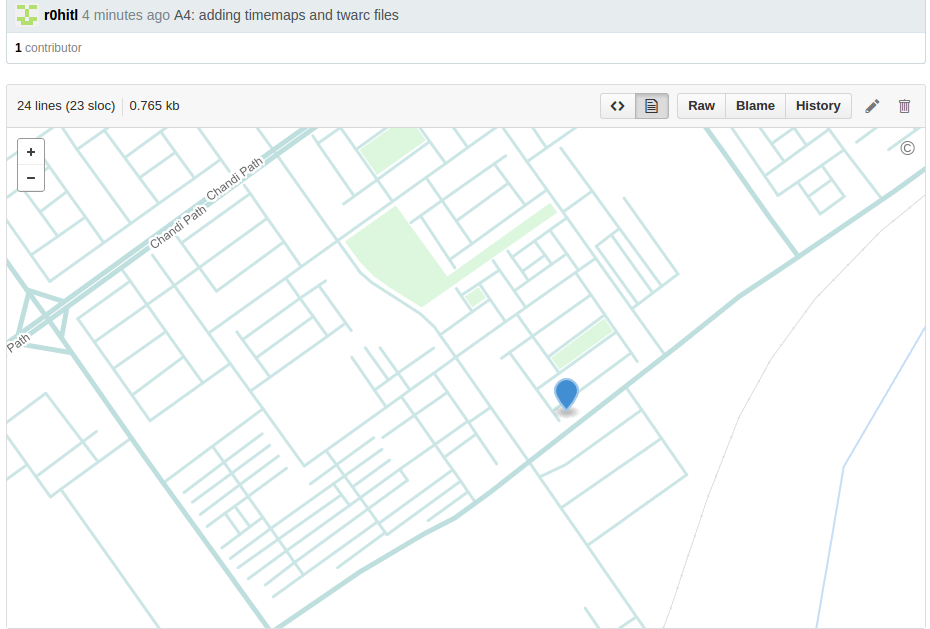
\includegraphics[scale=0.40]{graphs/gj1.png}
        \caption{GeoJSON 1}
    \end{center}
\end{figure}

\newpage
\begin{figure}[ht]    
    \begin{center}
        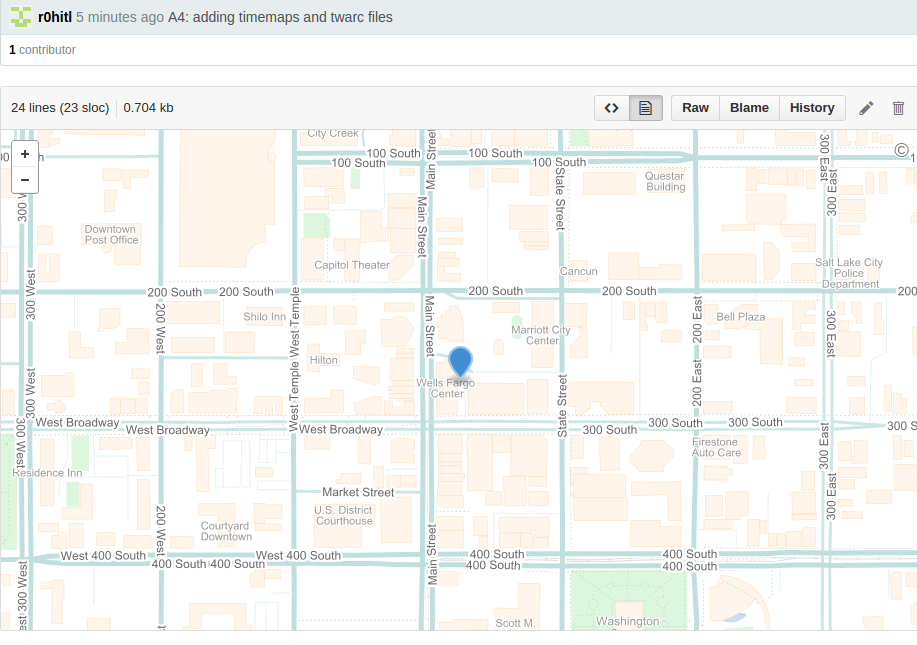
\includegraphics[scale=0.40]{graphs/gj2.png}
        \caption{GeoJSON 2}
    \end{center}
\end{figure}

\newpage
\begin{figure}[ht]    
    \begin{center}
        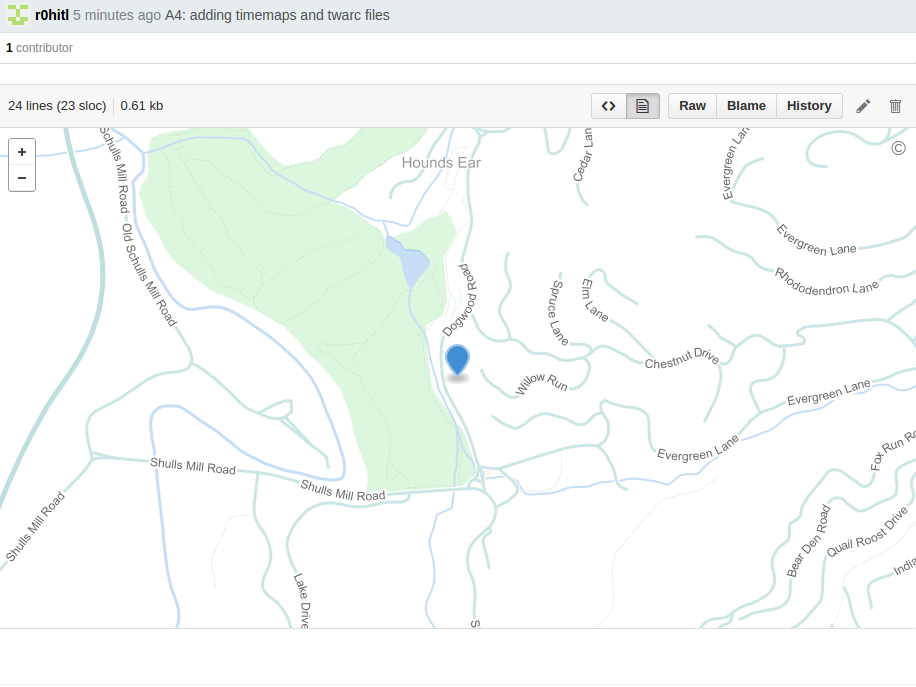
\includegraphics[scale=0.40]{graphs/gj3.png}
        \caption{GeoJSON 3}
    \end{center}
\end{figure}

\newpage
\begin{figure}[ht]    
    \begin{center}
        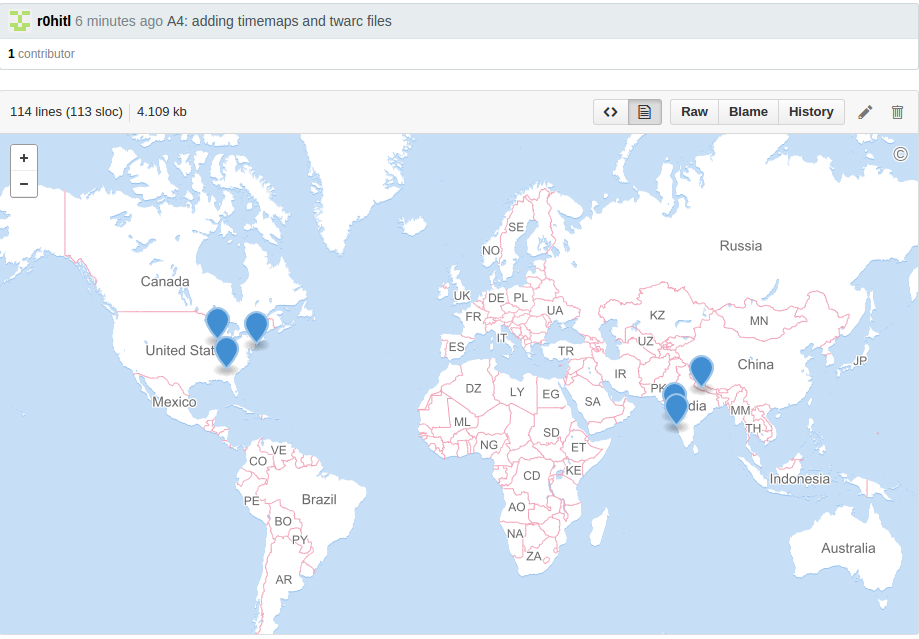
\includegraphics[scale=0.40]{graphs/gj4.png}
        \caption{GeoJSON 4}
    \end{center}
\end{figure}

\newpage
\begin{figure}[ht]    
    \begin{center}
        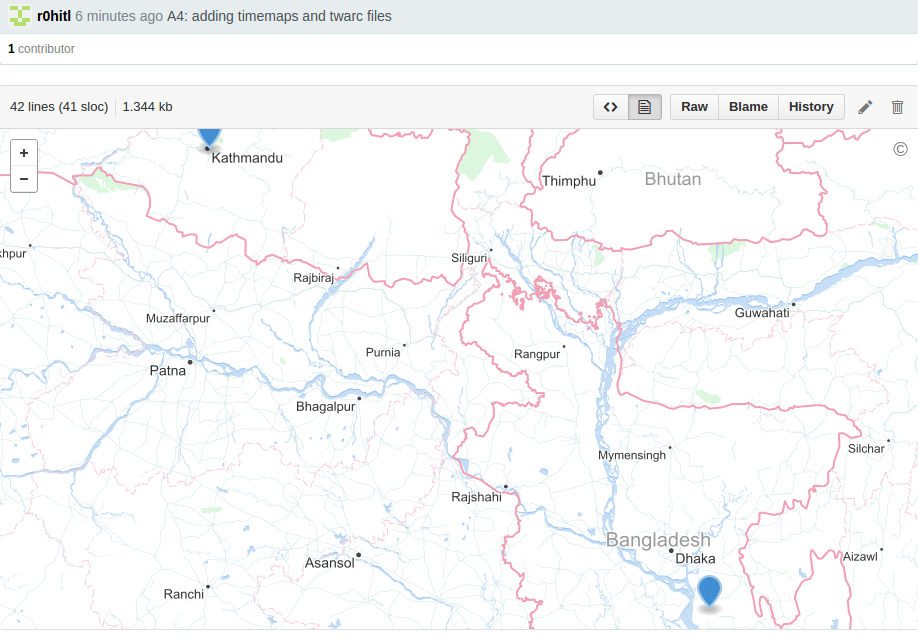
\includegraphics[scale=0.40]{graphs/gj5.png}
        \caption{GeoJSON 5}
    \end{center}
\end{figure}

\newpage
\subsection{Code Listing}
\subsubsection{Python program to fetch to fetch tweets using `twarc' library}
\lstinputlisting[language=Python,breaklines = true,frame=single, label=lst:q1-1,captionpos=b,numbers=left,showspaces=false,showstringspaces=false,basicstyle=\footnotesize]{src/4.tweetFetcherNepal.py}
\newpage

\end{enumerate}